\documentclass[border=3pt]{standalone}
% Preâmbulo compartilhado pelos diagramas TikZ da aula 13 (SLAM com EKF)
\usepackage[T1]{fontenc}
\usepackage[utf8]{inputenc}
\usepackage{lmodern}
\usepackage{amsmath}
\usepackage{xcolor}
\usepackage{tikz}
\usetikzlibrary{arrows.meta,angles,quotes,decorations.pathmorphing,decorations.pathreplacing,calc,
                positioning,shapes.geometric,shapes.misc,backgrounds,fit,
                math}

% Paleta (mesma dos SVGs originais)
\definecolor{dblue}{HTML}{2A5B8C}
\definecolor{dorange}{HTML}{B3541E}
\definecolor{dgreen}{HTML}{4A7C59}
\definecolor{dred}{HTML}{9C4B4B}
\definecolor{dcream}{HTML}{F4F1EA}
\definecolor{dshade}{HTML}{DDD7C9}

% Função gaussiana (não normalizada por padrão de escala visual)
\pgfmathdeclarefunction{gauss}{3}{%
  \pgfmathparse{1/(#3*sqrt(2*pi))*exp(-((#1-#2)^2)/(2*#3^2))}%
}

% Estilos comuns (prefixo d... para não colidir com chaves internas do pgf)
\tikzset{
  >={Stealth[length=2mm]},
  dguide/.style={gray!55, dashed, line width=0.4pt},
  daxis/.style={gray!60, line width=0.7pt, ->},
  dbody/.style={fill=black!3, draw=black!80, line width=1pt},
  dacc/.style={draw=dblue, line width=1pt},
  dlbl/.style={black!55, font=\small},
  dsub/.style={black!45, font=\footnotesize},
  dstate/.style={circle, draw=black!80, fill=dcream, line width=1pt,
                 minimum size=17mm, font=\large, inner sep=1pt},
  dobs/.style={circle, draw=black!80, fill=dshade, line width=1pt,
               minimum size=14mm, font=\large, inner sep=1pt},
  dbox/.style={rounded corners=2pt, draw=black!80, fill=dcream, line width=1pt,
               align=center, inner sep=6pt},
  dop/.style={circle, draw=black!80, fill=white, line width=1pt,
              minimum size=6mm, inner sep=0pt, font=\small},
  dtrans/.style={->, dblue, line width=1pt},
  dmeas/.style={->, dorange, line width=1pt},
  dcurve/.style={line width=1pt, dblue},
  dcurveb/.style={line width=1.4pt, dorange},
}

\begin{document}
\hyphenpenalty=10000 \exhyphenpenalty=10000 \tolerance=9999 \emergencystretch=3em
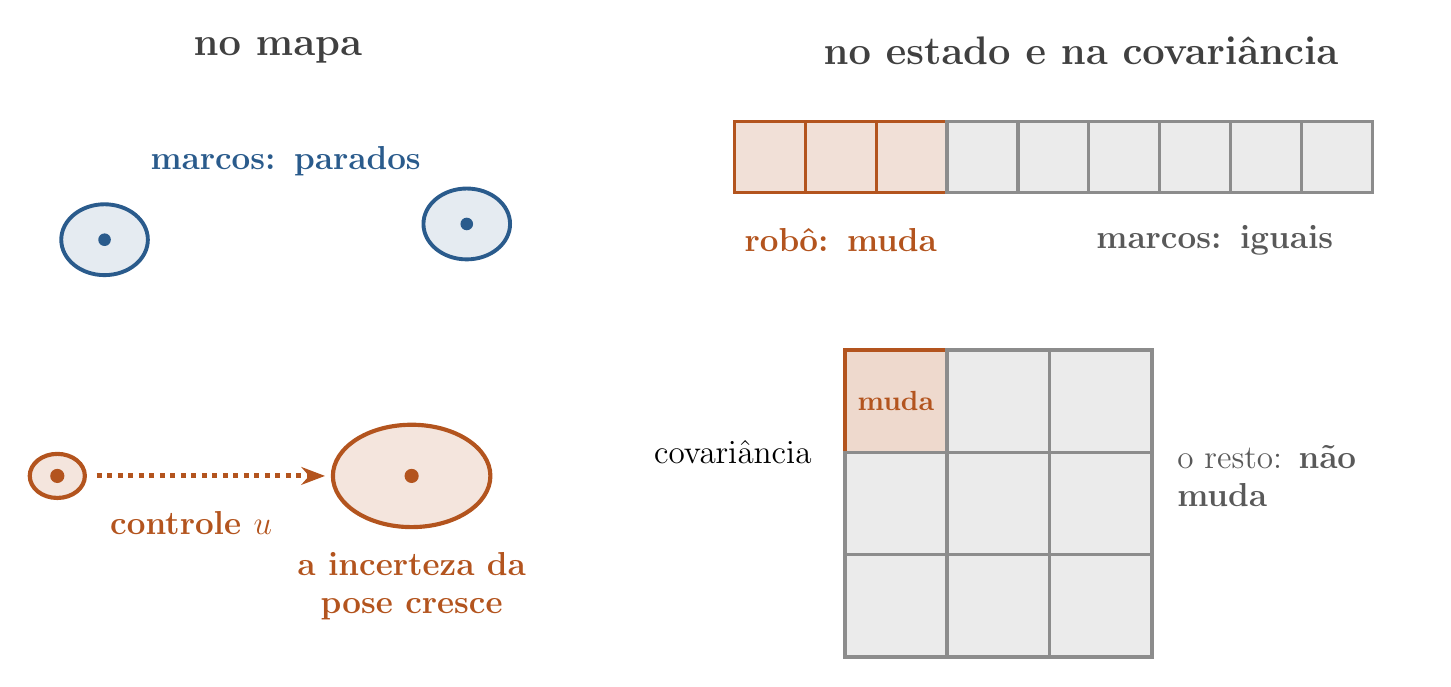
\begin{tikzpicture}[x=1cm,y=1cm]
\node[font=\Large\bfseries, black!75] at (4.4,8.4) {no mapa};
\draw[dorange, fill=dorange!15, line width=1.5pt] (1.6,3.0) ellipse (0.35 and 0.28); \fill[dorange] (1.6,3.0) circle (0.09);
\draw[dorange, dotted, line width=1.8pt, -{Stealth[length=3mm]}] (2.1,3.0) -- (5.0,3.0);
\node[font=\large\bfseries, dorange] at (3.3,2.4) {controle $u$};
\draw[dorange, fill=dorange!15, line width=1.5pt] (6.1,3.0) ellipse (1.0 and 0.65); \fill[dorange] (6.1,3.0) circle (0.09);
\node[font=\large\bfseries, dorange, text width=4cm, align=center] at (6.1,1.6) {a incerteza da pose \textbf{cresce}};
\draw[dblue, fill=dblue!12, line width=1.4pt] (2.2,6.0) ellipse (0.55 and 0.45); \fill[dblue] (2.2,6.0) circle (0.08);
\draw[dblue, fill=dblue!12, line width=1.4pt] (6.8,6.2) ellipse (0.55 and 0.45); \fill[dblue] (6.8,6.2) circle (0.08);
\node[font=\large\bfseries, dblue, text width=5cm, align=center] at (4.5,7.0) {marcos: \textbf{parados}};
\node[font=\Large\bfseries, black!75] at (14.6,8.4) {no estado e na covariância};
\draw[dorange, fill=dorange!18, line width=1.2pt] (10.2,6.6) rectangle (11.1,7.5);
\draw[dorange, fill=dorange!18, line width=1.2pt] (11.1,6.6) rectangle (12.0,7.5);
\draw[dorange, fill=dorange!18, line width=1.2pt] (12.0,6.6) rectangle (12.9,7.5);
\draw[black!45, fill=black!8, line width=1.2pt] (12.9,6.6) rectangle (13.8,7.5);
\draw[black!45, fill=black!8, line width=1.2pt] (13.8,6.6) rectangle (14.7,7.5);
\draw[black!45, fill=black!8, line width=1.2pt] (14.7,6.6) rectangle (15.6,7.5);
\draw[black!45, fill=black!8, line width=1.2pt] (15.6,6.6) rectangle (16.5,7.5);
\draw[black!45, fill=black!8, line width=1.2pt] (16.5,6.6) rectangle (17.4,7.5);
\draw[black!45, fill=black!8, line width=1.2pt] (17.4,6.6) rectangle (18.3,7.5);
\node[font=\large\bfseries, dorange, text width=3cm, align=center] at (11.55,6.0) {robô: \textbf{muda}};
\node[font=\large\bfseries, black!65, text width=5cm, align=center] at (16.3,6.0) {marcos: \textbf{iguais}};
\draw[dorange, fill=dorange!22, line width=1.3pt] (11.6,4.6) rectangle (12.9,3.3);
\draw[black!45, fill=black!8, line width=1.3pt] (12.9,4.6) rectangle (14.2,3.3);
\draw[black!45, fill=black!8, line width=1.3pt] (14.2,4.6) rectangle (15.5,3.3);
\draw[black!45, fill=black!8, line width=1.3pt] (11.6,3.3) rectangle (12.9,2.0);
\draw[black!45, fill=black!8, line width=1.3pt] (12.9,3.3) rectangle (14.2,2.0);
\draw[black!45, fill=black!8, line width=1.3pt] (14.2,3.3) rectangle (15.5,2.0);
\draw[black!45, fill=black!8, line width=1.3pt] (11.6,2.0) rectangle (12.9,0.7);
\draw[black!45, fill=black!8, line width=1.3pt] (12.9,2.0) rectangle (14.2,0.7);
\draw[black!45, fill=black!8, line width=1.3pt] (14.2,2.0) rectangle (15.5,0.7);
\node[font=\normalsize\bfseries, dorange] at (12.25,3.95) {muda};
\node[font=\large, black!65, anchor=west, text width=3cm] at (15.7,3.0) {o resto: \textbf{não muda}};
\node[font=\large, text width=4.6cm, align=right, anchor=east] at (11.3,3.3) {covariância};
\end{tikzpicture}
\end{document}
